\documentclass{article}
\usepackage{amsmath}
\usepackage{amssymb}
\usepackage{geometry}
\usepackage{graphicx}
\usepackage{hyperref}
\usepackage{graphicx}
\usepackage{caption}
\usepackage{subcaption}
\usepackage{amsmath}
\usepackage{float}
\usepackage{listings} 
\usepackage{color}

\title{Spectral Clustering From Scratch}
\author{Manthan Bagade, Anay}
\date{July 2025\thanks{Thanks to Coding Club, IITG for this assignment.}}

\begin{document}
\maketitle

\section{Introduction}
\label{sec:intro}
Spectral clustering is one of the unsupervised algorithms to group datapoints. In recent years, spectral clustering has become one of the most popular modern clustering
algorithms. It is simple to implement, can be solved efficiently by standard linear algebra software,
and very often outperforms traditional clustering algorithms, such as the k-means algorithm. \newline
Here we will implement a variant of this algorithm from scratch(using only numpy). We will go through various components of the algorithm and understand them one by one. We have implemented the algorithm with the help of Python classes. The notebook - \url{https://github.com/cryptic-mortal/from-scratch/tree/0a68dfdbaff1f1e0c20de611eb0d713b03400cd8/SpectralClustering_%26_GPR} contains the code, comparisons and visualizations of the algorithm.

\section{The need for spectral clustering}
\label{sec:need}
Spectral clustering is a powerful technique for clustering data that is not linearly separable. It helps us overcome two major problems in clustering: one being the shape of the cluster and the other being determining the cluster centroid. K-means algorithm generally assumes that the clusters are spherical or round, i.e. within k-radius from the cluster centroid. In K-means, the algorithm requires many iterations to determine the cluster centroid. \newline In spectral clustering, the clusters do not adhere to a fixed shape or pattern. The algorithm assigns points that are far apart but connected to the same cluster, while points that are close to each other could belong to different clusters if they are not connected. This suggests that the algorithm may be effective for data with varying shapes and sizes. These properties make spectral clustering a powerful tool for clustering data that is not linearly separable, and it has been shown to outperform traditional clustering algorithms in many cases. It is more efficient than k-means as it computes just the eigenpairs of the Laplacian matrix as discussed in \autoref{sec:laplacian}. However, it is important to note that spectral clustering can be sensitive to the choice of similarity measure and the number of clusters.

\begin{figure}[ht]
  \centering
  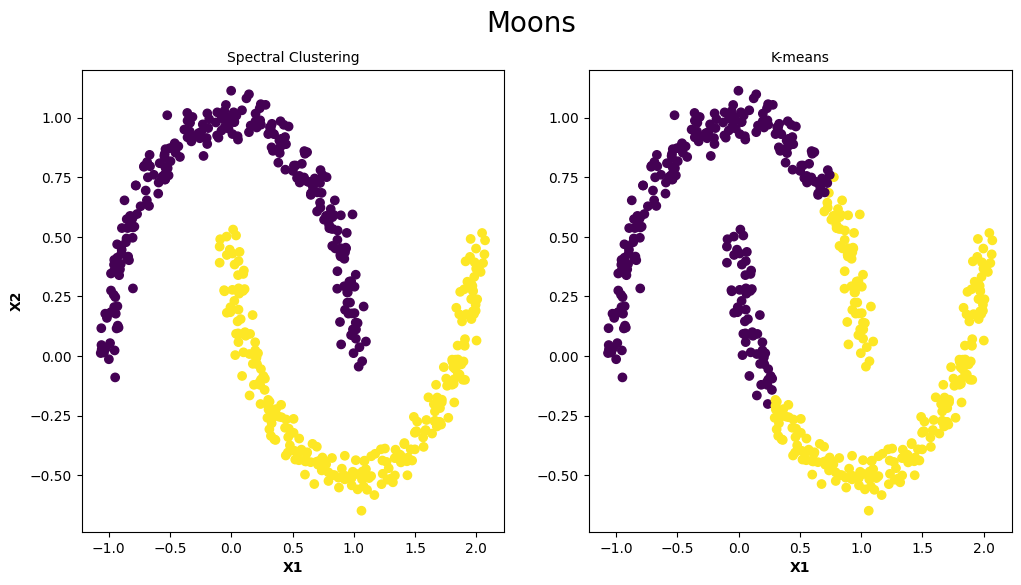
\includegraphics[width=0.8\textwidth]{images/comp.png}
  \caption{Comparison of Spectral Clustering and KMeans on the Moons dataset}
  \label{fig:comparison}
\end{figure}
Clearly, KMeans fails to cluster the data correctly, while spectral clustering does a good job of grouping the points based on their connectivity. Now let's understand the nitty-gritty of the algorithm.

\section{Adjacency Matrix and Similarity}
\label{sec:adjacency}
Given a set of data points $x_1, \ldots, x_n$ and some notion of similarity $s_{ij} \geq 0$ between all pairs of data points $x_i$ and $x_j$, the intuitive goal of clustering is to divide the data points into several groups such that points in the same group are similar and points in different groups are dissimilar to each other. There are several popular constructions to transform a given set $x_1, \ldots,x_n$ of data points with pairwise
similarities $s_{ij}$ or pairwise distances $d_{ij}$ into a graph. For this implementation, we will use the adjacency matrix $A$ which is defined as follows:



\begin{equation}
s_{ij} =
\begin{cases}
e^{-\dfrac{\|x_i - x_j\|^2}{2\sigma^2}} & \text{if } i \ne j \\
0 & \text{if } i = j
\end{cases}
\end{equation}
Here, $\sigma$ is a hyperparameter that controls the connectivity of the datapoints. The greater the value of sigma, the more connected the points become,i.e, it increase the global connectivity of the graph.
\begin{figure}[ht]
  \centering
  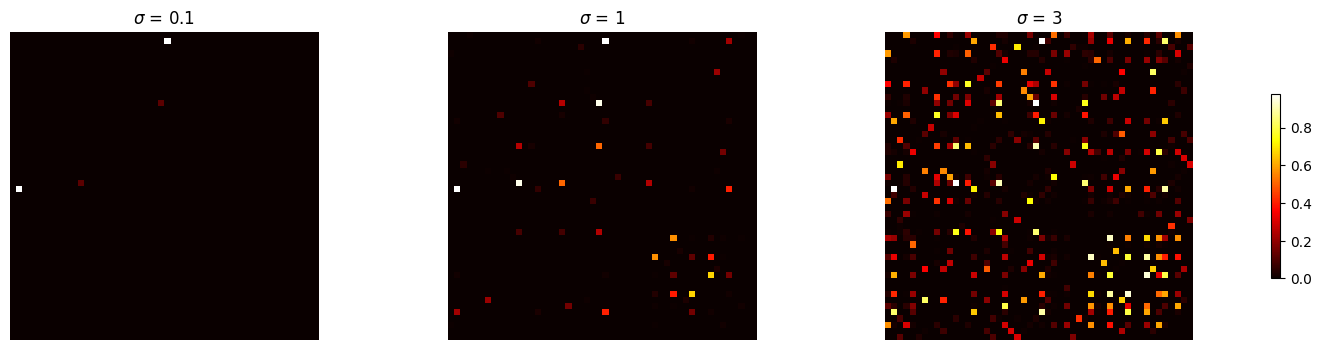
\includegraphics[width=1.0\textwidth]{images/sigma_comp.png}
  \caption{Comparison of $\sigma$ values on the moons dataset}
  \label{fig:sigma_comparison}
\end{figure} 
\newline

The adjacency matrix $A$ is then constructed from the similarity matrix $S = (s_{ij})$ as follows:
\begin{equation}
A_{ij} = \begin{cases}
s_{ij} & \text{if } s_{ij} > 0 \\
0 & \text{otherwise}
\end{cases}
\end{equation}

\section{Degree Matrix}
\label{sec:degree}
The degree matrix $D$ is a diagonal matrix that contains the sum of the weights of the edges connected to each vertex in the graph. $D$ represents the total connection strength of node i to all other nodes. The higher the value of $D_{ii}$, the higher the node $i$ is connected to other nodes and the strongly it is connected. It is defined as follows:
\begin{equation}
D_{ii} = \sum_{j=1}^{n} A_{ij}
\end{equation}

\section{Laplacian Matrix}
\label{sec:laplacian}
The Laplacian matrix $L$ also known as Graph Laplacian is a matrix representation of a graph that captures the connectivity of the graph. We use the Laplacian matrix to transform the data into a lower-dimensional space ($k$ dimensional) where the clusters can be easily separated. You select the first k eigenvectors corresponding to the smallest eigenvalues except the \textbf{trivial eigenvalue - 0}. The eigenvectors of $L$ are sorted in ascending order of their eigenvalues, as the smallest eigenvalues give smooth, broad pattern and are not sensitive to noise. Here, we are going to use \textbf{Normalized Graph Laplacian}. It has several advantages :
\begin{enumerate}
\item Since it is symmetric, it has real, positive eigenvalues and orthogonal eigenvectors.
\item It is invariant to the scaling of the graph, i.e., avoids letting high degree nodes dominate the clustering.
\item Numerically stable due to normalization.
\end{enumerate}
The normalized Laplacian matrix is defined as:
\begin{equation}
L = I - D^{-1/2} A D^{-1/2}
\end{equation}
where $I$ is the identity matrix, $D$ is the degree matrix, and $A$ is the adjacency matrix. We normalize the unnormalized Laplacian matrix with the matrix $D$.
\begin{equation}
L_{unnormalized} = D - A
\end{equation}
The normalized Laplacian matrix is then given by:
\begin{align*}
L_{\text{sym}} 
&= D^{-1/2} L_{\text{unnormalized}} D^{-1/2} \\
&= D^{-1/2} (D - A) D^{-1/2} \\
&= I - D^{-1/2} A D^{-1/2}
\end{align*}

\section{The Final Steps}
\label{sec:final}
Once we have the Laplacian matrix, we can compute the eigenvalues and eigenvectors of the Laplacian matrix. The eigenvectors corresponding to the smallest $k$ eigenvalues (excluding the trivial eigenvalue 0) are used to form a new matrix $X$ of size $n \times k$, where $n$ is the number of data points and $k$ is the number of clusters. The rows of this matrix represent the data points in the new space. We then apply a clustering algorithm, such as k-means, to the rows of this matrix to obtain the final clusters. The k-means algorithm is applied to the rows of the matrix $X$ which are datapoints in the new space.

\section{Implementation}
\label{sec:implementation}
The implementation of spectral clustering is done using Python classes. The name of the class is \texttt{SpectralClustering}, which takes the number of clusters \texttt{n\_clusters} and scaling parameter \texttt{sigma} as inputs. You can call \texttt{fit\_predict} method to fit the model and store the labels in a variable. Here is the implementation of the class:

\lstset{
  language=Python,
  basicstyle=\ttfamily\small,
  breaklines=true,           
  breakatwhitespace=true,    
  captionpos=b,              
  showstringspaces=false,   
  keywordstyle=\color{blue},
  commentstyle=\color{green},
  stringstyle=\color{red}
}
\begin{lstlisting}[caption={Spectral Clustering Implementation}, label={code:spectral}]
class SpectralClustering :

  def __init__(self, n_cluster, sigma = 1.0) -> None:
    self.n_cluster = n_cluster
    self.sigma = sigma
    self.labels_ = None

  def compute_affinity_matrix(self, X) -> np.ndarray:
    affinity_matrix = np.exp(-squareform(pdist(X, 'sqeuclidean'))/(2*self.sigma**2))
    np.fill_diagonal(affinity_matrix, 0)
    return affinity_matrix

  def compute_degree_matrix(self, affinity_matrix) -> np.ndarray:
    degree_matrix = np.diag(np.sum(affinity_matrix, axis=1))
    return degree_matrix

  def compute_laplacian_matrix(self, degree_matrix, affinity_matrix) -> np.ndarray:
    diag = np.diag(degree_matrix)
    diag = np.diag(1/np.sqrt(diag+1e-8))
    laplacian_matrix = np.eye(diag.shape[0]) - (diag @ affinity_matrix @ diag)
    return laplacian_matrix

  def compute_eigenvectors(self, laplacian_matrix) -> np.ndarray:
    eigenvalues, eigenvectors = eigh(laplacian_matrix)
    return eigenvectors[:,1:self.n_cluster+1]

  def fit(self, X) -> None :
    affinity_matrix = self.compute_affinity_matrix(X)
    degree_matrix = self.compute_degree_matrix(affinity_matrix)
    laplacian_matrix = self.compute_laplacian_matrix(degree_matrix, affinity_matrix)
    eigenvectors = self.compute_eigenvectors(laplacian_matrix)
    eigenvectors = eigenvectors / (np.linalg.norm(eigenvectors, axis=1,keepdims=True)+1e-8)
    kmeans = KMeans(n_clusters=self.n_cluster, random_state=0).fit(eigenvectors)
    self.labels_ = kmeans.labels_

  def fit_predict(self, X) -> np.array:
    self.fit(X)
    return self.labels_
\end{lstlisting}

\section{Results}
\label{sec:results}
We have tested the implementation on two datasets - Moons and Circle. The results are shown in \autoref{fig:spectral_clustering_result} and \autoref{fig:spectral_clustering_result_circle}. The implementation is able to cluster the points correctly in both cases.

\begin{figure}[ht]
\centering
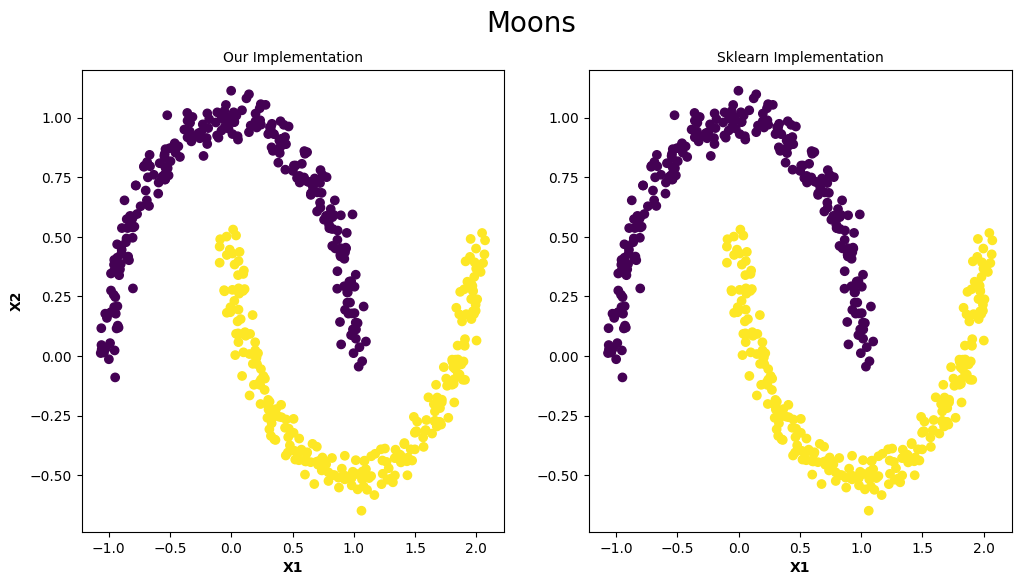
\includegraphics[width=0.8\textwidth]{images/moons_comp.png}
\caption{Spectral Clustering on Moons Dataset}
\label{fig:spectral_clustering_result}
\end{figure}

\begin{figure}[H]
\centering
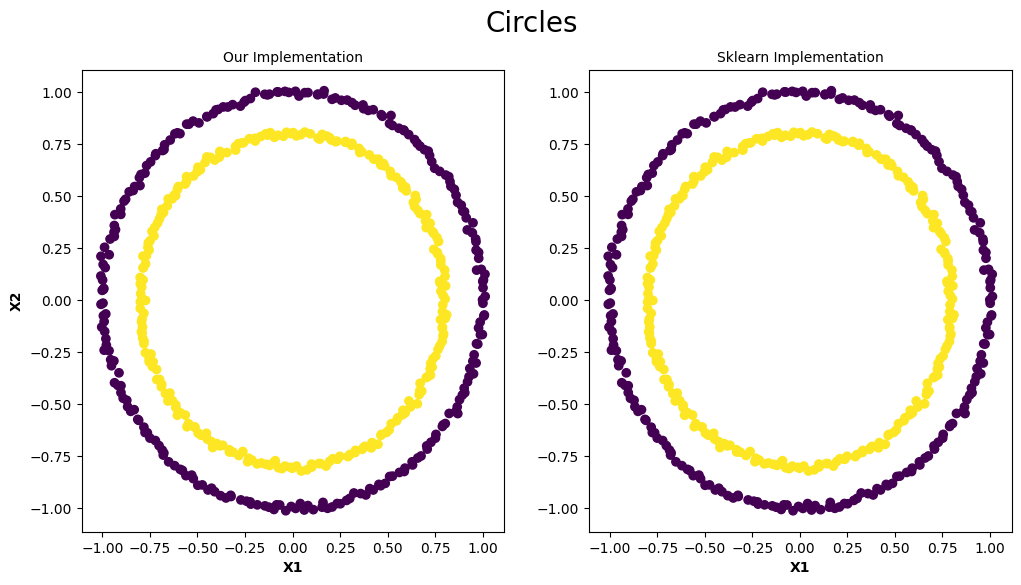
\includegraphics[width=0.8\textwidth]{images/circle_comp.png}
\caption{Spectral Clustering on Circle Dataset}
\label{fig:spectral_clustering_result_circle}
\end{figure}


\begin{thebibliography}{9}
\bibitem{greatleanring}
\href{https://www.mygreatlearning.com/blog/introduction-to-spectral-clustering/}{\textit{Introduction to Spectral Clustering}}, by Marina Chatterjee, July 25, 2024.
\bibitem{mit.edu}
\href{https://people.csail.mit.edu/dsontag/courses/ml14/notes/Luxburg07_tutorial_spectral_clustering.pdf}{A Tutorial on Spectral Clustering}, by Ulrike von Luxburg, 2007.
\bibitem{analyticsvidhya}
\href{https://www.analyticsvidhya.com/blog/2021/05/what-why-and-how-of-spectral-clustering/}{\textit{Spectral Clustering : A comprehensive guide for begineers}}, by Keerthana, Oct 14, 2024.
\bibitem{gfg}
\href{https://www.geeksforgeeks.org/machine-learning/ml-spectral-clustering/}{\textit{Spectral Clustering in Machine Learning}}, GeeksforGeeks article, July 12, 2025.
\bibitem{medium}
\href{https://rahuljain788.medium.com/implementing-spectral-clustering-from-scratch-a-step-by-step-guide-9643e4836a76}{\textit{Implementing Spectral Clustering from Scratch: A Step-by-Step Guide}}, by Rahul Jain, May 23 2024.
\bibitem{drdatascience}
\href{https://youtu.be/YHz0PHcuJnk?si=TLcduWA458duAHzX}{\textit{3 easy steps to understand and implement spectral learning in python}}, by Dr. Data Science, May 30, 2021.
\bibitem{ronandmath}
\href{https://youtu.be/uTUVhsxdGS8?si=8sFtW-p11xJVOAMI}{Spectral Graph Theory for Dummies}, by Ron and Math, May 16, 2024.

\end{thebibliography}

\end{document}      